\documentclass{article}
\usepackage[utf8]{inputenc}

\title{Software Development Lifecycle Plan}
\author{Maxwell Sweikart, Nina Yakovchits, Ryan Castner}
\date{April 2015}

\usepackage{graphicx}
\graphicspath{ {images/} }
\usepackage{hyperref}
\hypersetup{colorlinks=true, urlcolor=cyan}
\begin{document}

\maketitle

\section{Introduction}
The purpose of this document is to discuss the merits and flaws of the chosen Software Development Life Cycle (SDLC) our team will follow while refactoring the Edge Diagrammer application.
\hfill \\

\section{Software Development Lifecycle Approaches}
The following is a list of common Software Development Life Cycles: \hfill \\
\begin{enumerate}
\item Waterfall Model
\item Spiral Model
\item Top-Down Model
\item Bottom-Up Model
\item Hybrid Model
\item Rapid Prototyping
\item Object-Oriented Model
\item Iterative Model
\item Big Bang Model
\item V-Model
\end{enumerate}

This list is by no means exhaustive, but includes life cycles that are common and familiar with the team. Above were the initial candidates for a SDLC to follow. Our team quickly narrowed down the options due to our desire to have a Test-Driven approach. A goal of our project is to strictly refactor the code and thus our test suite will ensure that we do not change the expected functionality of the existing methods in the application. We quickly crossed out the Waterfall and V-Model because they would only allow for testing during certain stages of the cycle and not continuously on each build of the refactored application. Out of the remaining models we quickly discerned that many approaches were tailored to the creation of software including eliciting requirements, planning, deployment, and maintenance. Since we are coming into this with a mindset of rapidly refactoring and testing code to include new functionality and increase extensibility while maintaining a Test-Driven approach we decided to go with the Iterative Model. \hfill \\

\section{Argument for the Iterative Approach}
The Iterative Model is an approach defined by the implementation of a small set of requirements that is tested, implemented, and then iterated on to extend and enhance those features and add new ones.

\begin{figure}[h]
\caption{Example of an Iterative Approach}
\centering
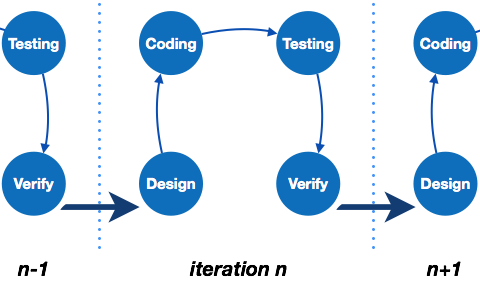
\includegraphics[scale=0.5]{sdlc_iterative}
\end{figure}


As a team we thought this would be the best approach to the work we would be doing because it incorporates a "smoke test" of sorts at the end of each iteration where we can implement the goals outlined in our testing plan. Furthermore as we continue to refactor we can ensure at each step in the process we have maintained existing external functionality. Overall, the Iterative Model works well because the requirements are well defined at the outset but allow room for evolution over time -- e.g. increasing extensibility and how this might be interpreted -- naturally lends itself to an iterative approach to development.\hfill \\

One of the main flaws of the iterative approach is that given a smaller project, the ability to break down the project into smaller chunks to iterate over becomes increasingly difficult. This issue is not a concern with this project however, there are many modules that interact in different ways, and much room for growth and expansion as the definitions of refactoring and increasing extensibility are quite broad. The second main flaw is that if the requirements at the start of the project were not well-defined there would be a major setback in the development cycle. Again though, due to the rigid definitions and scope of this project this should not be an issue.

\section{Defining the Current System Schema}
To aid with the concept of refactoring we have designed a flow of the current system modules and how they interact with one another. The model as defined below provides us with a basis for how the current system works and allows us to ensure that the addition of any new modules to increase extensibility do not affect the current structure and flow of the application.

\begin{figure}[h]\raggedleft
\caption{Flowchart of the current application}
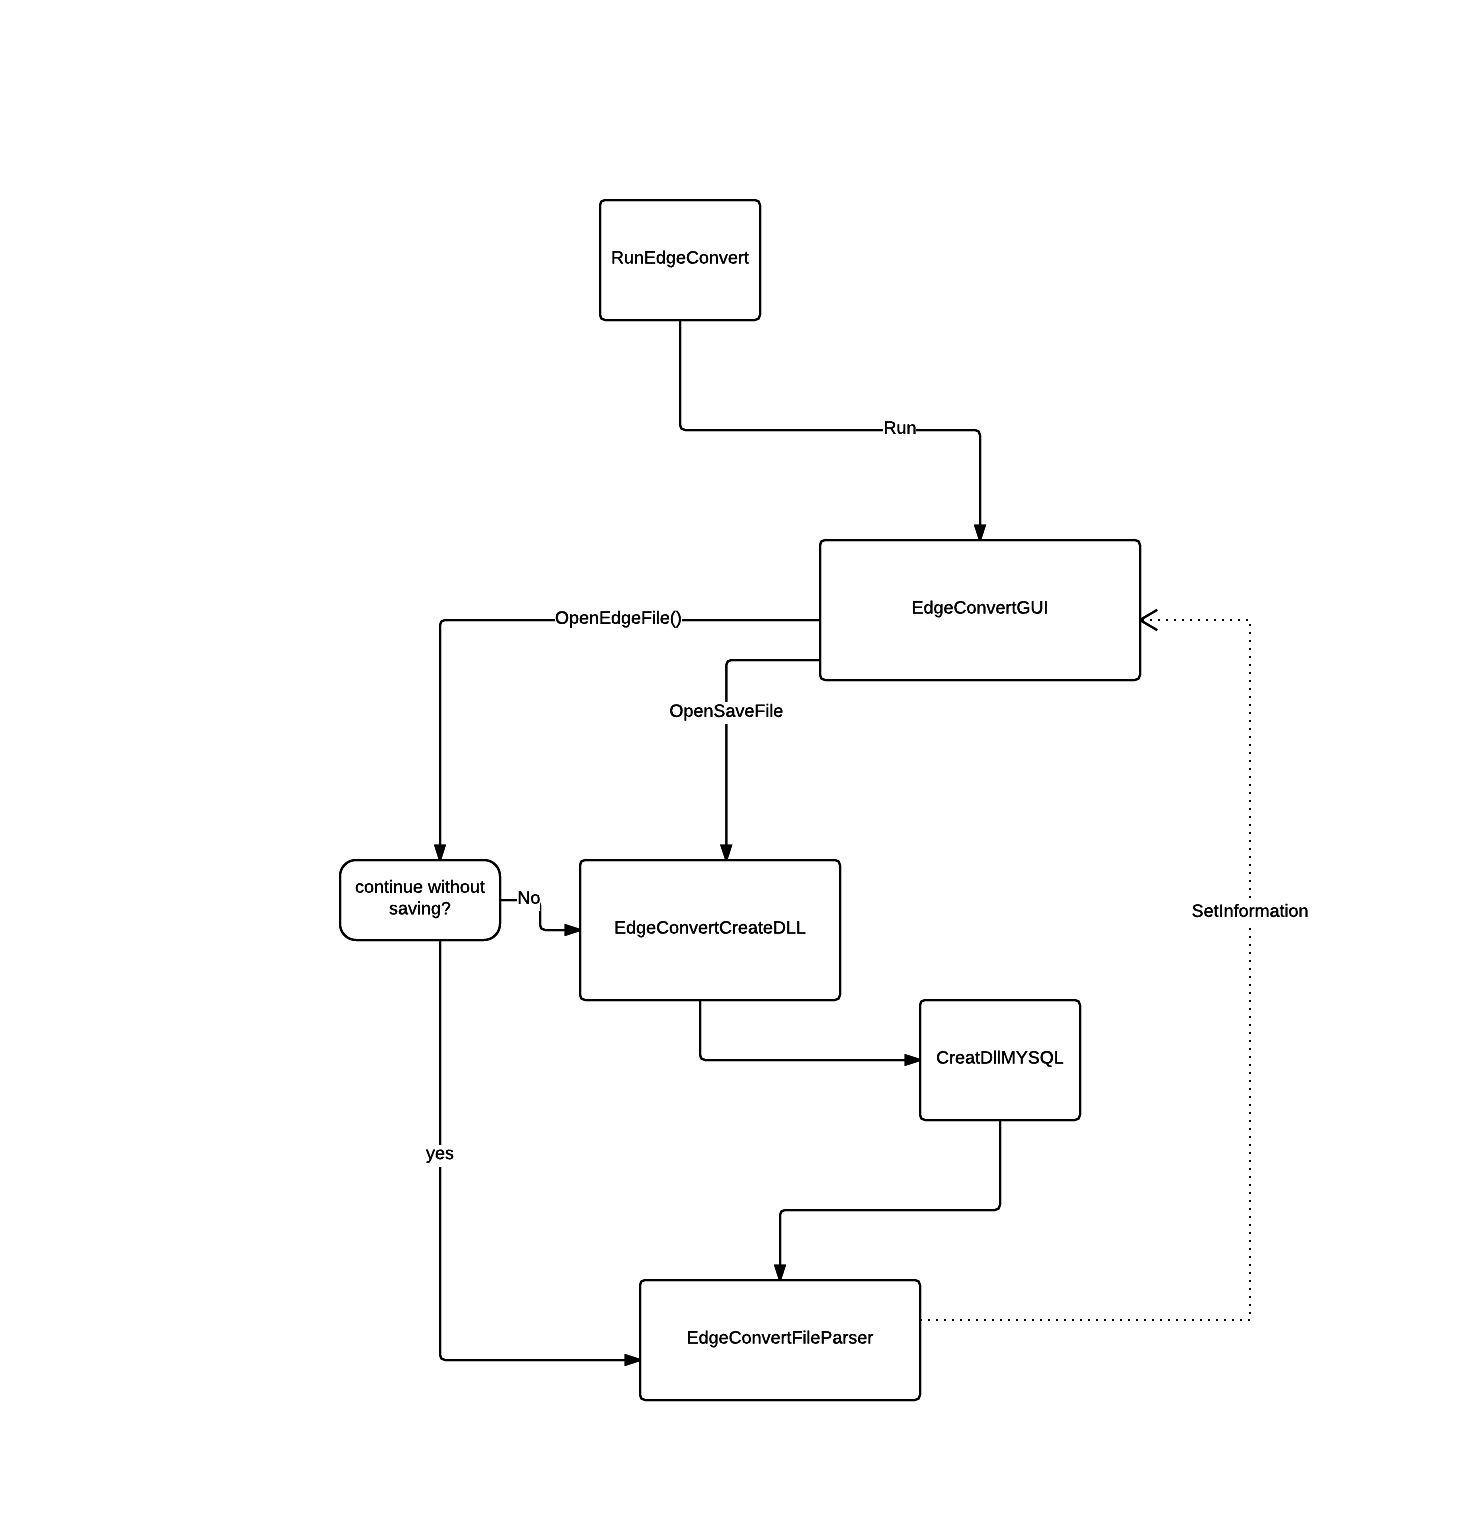
\includegraphics[scale=0.75]{InitialApplicationFlow}
\end{figure}

\end{document}